\documentclass[a4paper, 12pt]{report}
% list options between brackets
\usepackage{graphicx, url, placeins, algorithm, algorithmic, hyperref, wrapfig, amsmath, lipsum, cite, caption, subcaption}
\graphicspath{{figures/}}
\newcommand{\squeezeup}{\vspace{-2.5mm}}

\usepackage{titlesec, color}

\definecolor{gray75}{gray}{0.75}
\newcommand{\hsp}{\hspace{10pt}}

\titleformat{\chapter}[hang]{\Huge\bfseries}{\thechapter\hsp\textcolor{gray75}{|}\hsp}{0pt}{\Huge\bfseries}
\titlespacing*{\chapter}
  {0pt}{-70pt}{20pt}

\begin{document}

\title{Monte Carlo-based ray tracer\\ Project Report}   % type title between braces
\author{
	Johan Beck-Nor\'{e}n, johbe559@student.liu.se
	\\Andreas Valter , andva287@student.liu.se
	}
\date{\today}    % type date between braces
\maketitle

\setcounter{page}{2}
\begin{abstract}
This report describes the techniques required to approximate global illumination in a computer generated scene and is created as a result from the course TNCG15, Advanced Global Illumination and Rendering.
The report focus on the techniques required to do a monte-carlo ray tracer and show results from our implementation using that technique.
It will cover topics like intersection testing, aliasing counter actions and other techniques that has been implemented during the project.
The results presentated will evaluate these parts, both to see their contributions and to show the time cost that is added when using them.

\end{abstract}

\tableofcontents


\chapter{Introduction} \label{ch:introduction}
Realistic lighting in computer graphics scenes has been a problem for many years. 
The equation describing light propagation trough a scene is both recursive and infinite which is definitely something that computers can not currently handle.
Therefore, researchers has found different methods to estimate the analytic solution.
These methods use iterations, using computer power to calculate these estimates that converge towards the real solution.\\

Most of these are so called ray tracing methods where rays are traced from the viewer into the scene.
When rays hits surfaces in the scene, new rays for reflection and refraction is spawned.
These are then combined using importance.

\section{Whitted ray tracing}
The Whitted ray tracing method described by Turner Whitted in \cite{Foley_animproved} was the first global illumination method that took the whole scene into consideration when calculating intensity values.
In previous so called ray marching solutions, the calculations stopped as a ray hit a surface and local lightning models like Lambert's cosine rule to model perfectly diffuser or the Phong model. \\

\begin{equation} \label{eq:phong}
\emph{I} = \emph{I}_{a} + \emph{k}_{d} \sum_{j=1}^{j=ls} (  \mathbf{N} \cdot \mathbf{L}_j) + \emph{k}_{s} \sum_{j=1}^{j=ls} (  \mathbf{R}_j \cdot \mathbf{V})^n
\end{equation}

The Phong model given by \autoref{eq:phong} is a local light model.
It assumes that each light source $\emph{L}_j$ is located at a point with infinite distance to the objects in the scene. 
The total reflected intensity $\emph{I}$ is calculated using the reflection due to ambient light $\emph{I}_{a}$ together with two terms, one term for diffuse light and one specular term.
The two constants $\emph{k}_{d}$ and $\emph{k}_{s}$ is reflection constants that regulates their contributions.
The diffuse term uses the Lamberts cosine law to describe the color using a dot product between the normal and the light direction to calculate if that part of the surface is directed towards the light source.

The specular term uses the direction that a perfect reflection $ \bar{V} $ from the light source would take on the surface together with a ray towards the viewer $\bar{V}$.\\

Whitted extended the previous techniques and allowed for rays to bounce in the scene and thus creating the basis for global illumination.
The solution he presented allowed for true reflections, shadows and refractions.
By using the Phong model on each ray hit and spawning new rays recursively for reflections, shadow rays and refractions a method for simulating global lightning is created.

When using several rays in the scene, a term importance is introduced.
It states that the total importance of all rays for each pixels is one. 
If multi sampling is used, importance is divided among the rays.
The importance flows in the opposite direction as the light, from the camera and into the scene.

\section{Radiosity}
Radiosity is an algorithm for global illumination which only handles diffusely reflected light, and is therefore not dependent on any camera position or direction. This means that the solution converges toward a steady state, and can for example be pre-computed for use in static scenes. The algorithm works by splitting the scene geometry into a number of finite area elements called patches, and solves the rendering equation for surfaces that diffusely reflects light. A visibility factor, called \emph{form factor}, is used to describe a patch's visibility toward all other patches in the scene. The size of a view factor is dependent on the distance between any two patches, their orientation in relation to each other, partial or total occlusion etc. and describes the amount of radiance leaving a patch $j$ arriving at patch $i$ for all patches $j \in N$ for a scene consisting of $N$ number of patches. The form factors make up a system of linear equations, which when solved produces the radiosity for each patch. The process can be iterated to perform several passes and allowing for multiple bounces to be computed.

\section{Monte Carlo ray tracing}
A rendering equation (\ref{eq:rendering_eq}) presented by Kajiya in \cite{kajiya} describes a full global illumination solution for a given scene. It is an integral equation called a Fredholm equation of the second kind because of the unknown radiance quantity, $L(...)$, appears on both sides of the equation. This makes the equation a recursive one, corresponding to a ray's multiple bounces through a scene. It is described below using the same notation as Dutr\'{e} et al. in \cite{dutre}, and we will use this notation throughout this report.
\begin{equation}
\label{eq:rendering_eq}
\begin{split}
L(x \rightarrow \theta) = L_e(x \rightarrow \theta) + L_r(x \rightarrow \theta) =\\ 
L_e(x \rightarrow \theta) + \int_{\Omega_x} f_r(x, \Phi \rightarrow \theta)L(x \leftarrow \Phi)cos(N_x, \Phi)d\omega_{\Phi}
\end{split}
\end{equation}
The Monte Carlo integration method introduces a method for calculating an estimated value for an integral expression. This is done by sampling the integral function by random discreet numbers, and as the number of samples increase the produced solution's accuracy increases as well.

\begin{equation}
 \label{eq:monte_carlo_example1}
 I = \int f(x) dx
 \end{equation}
 \begin{equation}
 \label{eq:monte_carlo_example2}
 \langle I \rangle = \frac{1}{N} \sum^N_i \frac{f(x_i)}{p(x_i)} dx
 \end{equation}
 The intergral in \autoref{eq:monte_carlo_example1} with a value of \emph{I} can me \emph{estimated} as in equation \autoref{eq:monte_carlo_example2} as $\langle I \rangle$ by $N$ number of samples distibuted according to the pdf $p(x_i)$. 
 This method will later be used to estimate the solution to \autoref{eq:rendering_eq}.\\

-Similar to a Whitted ray tracer, a Monte Carlo ray tracer starts by shooting rays from a virtual camera through a view plane into the scene. 
One difference is that Monte Carlo ray tracing handles diffuse interreflections and specular-diffuse surface interreflections, color bleeding between objects, and soft shadows by sampling area light source surfaces for each ray intersection. 
As the number of samples increase the more accurate the integral estimation will be, and the algorithm produces noise if the number of samples are too low. 
There are several ways to reduce the noise. 
One could separate the calculations for direct and indirect illumination, using shadow rays to more quickly compute direct diffuse illumination and soft shadows. 
Sampling directions for diffuse indirect illumination could be chosen in more informed ways to reduce the noise. 
There have also been research on methods combining the benefits of radiosity with the benefits of ray tracing.

\section{Two-pass rendering}
Since a radiosity method handles diffuse reflections rather well, and a ray tracing method handles specular reflections well. a lot of research has been done to find ways to combine these two methods.
One of these methods descibed by Smits et al. \cite{importance_radiosity} works from the fact that radiosity algorithms propagate light from a light source through the scene, while a ray tracing algorithm only cares about the light that reaches the eye.
The method in \cite{importance_radiosity} consists of splitting the rendering into two passes.
The first pass uses a ray tracing approach to emmit importance from the eye through the scene.
This importance is then used to refine the patches used for the second pass, a radiosity pass.
By subdividing patches in parts with high importance, and ignoring patches in areas with little or no importance, great speedups can be achieved.
 

\section{Photon mapping}
Monte carlo methods for ray tracing suffers from noise in the final results if not enough samples are used when calculating radiance from diffuse indirect illumination.
Photon mapping is two-pass global illumination method presented by Jensen \cite{photon_maps} which computes diffuse indirect illumination faster than a Monte Carlo solution.
The method works by emitting packets of energy (light) from the light sources toward different objects in the scene.
Different packets can be used for different materials, e.g. a high resolution photon map can be used for caustics that are visualized directly, while a lower resolution map can be stored for later use in the ray tracing step.
Shadow photons can be used to more efficiently compute shadows, and be used as directional information to produce more accurate sampling directions during the rendering step.
The method has been shown to reduce rendering time as well as the noise in the final image when used in a Monte Carlo ray tracer algorithm.
  
\section{Iso surface ray tracing}
An iso surface is a surface described implicitly by a mathematical expression or equation. An iso surface representation of a scene is preferable over polygonal objects in a ray tracing context for a few reasons. Implicitly described primitives and objects usually scale well if the resolution or precision of the illumination algorithm should increase, since they are not bound by a finite number of triangles, but rather a mathematical description. They are also easy to define and describe, and are rather straight-forward to calculate ray intersections against. From an intersection calculation we need to decide weather a ray is intersecting the surface, and if so at what position, and what is the normal vector for the surface at that position. 

\chapter{Background} \label{ch:background}

In this section we will talk about the methods we have implemented in our Monte Carlo ray tracer using C++. 
Although there are several approaches to some of these methods we will only talk about the methods we chose to implement in this project.

\section{Scene storage}
When calculating global illumination for the scene, all objects need to be taken into consideration when calculating the illumination for one part of the scene due to the recursive nature of \autoref{eq:rendering_eq}.

For ray tracing solutions, this means that as rays bounce inside the scene the first intersecting object needs to be located.
A na\"{\i}ve solution would be to store all objects without any information about where in the scene they are located.
When traversing a ray through the scene, the algorithm would have to check against all objects, even if almost all of the checks would be misses.
For a simple scene with only a few implicit objects this is a good solution. The overhead when dealing with an more complex storage method would make it slower than simply checking against all objects in the scene.
But when using a more complex scene consisting of models with hundreds of thousands of elements, it is possible to take advantage of the spatial information of each element to subtract a small subset and only do collision tests against those.

There are several methods for storing the scene using different techniques.

\subsection{Bounding box}
An axis aligned bounding box is an essential part of most scene storage methods.
This is the smallest box with its axes aligned to the Cartesian coordinates axes that can encapsulate the primitive that owns the bounding box.
The bounding box will not be the smallest box that can encapsulate the primitive but the intersection tests are much simpler compared to doing collision tests against arbitrarily rotated primitives.

\subsection{Bounding volume hierarchy}
Bounding volume hierarchy (BVH) uses a tree structure with bounding volumes like axis aligned bounding boxes. 
Small sets of primitives are divided into different bounding volumes.
These small volumes are then combined to larger bounding volumes recursively until there is only one bounding volume left surrounding the entire scene.
By using this technique, it is known that if the ray does not intersect a larger bounding box, the child boxes within that larger box can be ignored as well.

\subsection{Octree}
The octree method uses the bounding boxes in a slightly different way than described in the previous section.
The scene is encapsulated into a large bounding box.
When each primitive is added, the scene bounding box is subdivided into eight sub-volumes recursively until the current level of bounding boxes are to small to fit the primitive.
The primitive is then added to the level above that as a leaf.
Using this structure, it is possible to traverse the ray through the volume and, just as when using the BVH tree, large parts of the tree can be ignored by checking only parent nodes for intersection.

\section{Intersection}
The implementation needs to be able to handle several different intersection algorithms, one for each type of primitive in the scene.
To make sure that all kinds of primitives are supported, inheritance is used where each primitive inherits from an abstract class.
During rendering calculation, the ray tracer calls an abstract method for calculation of intersection points on the given primitive and therefore the implementation supports all primitives that can define a intersection method.
Each of these methods uses an incoming ray with a direction vector $d$ and a origin $o$ described by \autoref{eq:ray}.
The intersection methods has to calculate the normal of surfaces to decide the direction of new rays spawned at the intersection point.
\begin{equation} \label{eq:ray}
\mathbf{p} = \mathbf{o} + t \mathbf{d}, t \geq 0
\end{equation}

\subsection{Implicit sphere}
A sphere is defined by a position vector $c$ of its centre and a radius scalar $r$. 
The goal is to find if any $t$ in \autoref{eq:ray} satisfies \autoref{eq:sphere}. By inserting \autoref{eq:ray} into \autoref{eq:sphere}, we receive an expression for solving the intersection point described by \autoref{eq:sphereray}.
\begin{equation} \label{eq:sphere}
(\mathbf{p} - \mathbf{c}).(\mathbf{p} - \mathbf{c}) = r^2
\end{equation}

\begin{equation} \label{eq:sphereray}
(\mathbf{d} \cdot \mathbf{d})t^2 + 2(\mathbf{o} - \mathbf{c}) * \mathbf{d} t + (\mathbf{o} - \mathbf{c}) \cdot (\mathbf{o} - \mathbf{c}) - r^2=0
\end{equation}

There are two solutions to \autoref{eq:sphereray} described in \autoref{eq:sparsol} with coefficients described by \autoref{eq:sparsub}.
When intersecting, they represent the entry and exit point on the sphere surface.
The collision point is decided dependent on if the solution is real, this means that $B^2 - 4 A C >= 0$ is true for all rays that collide with the sphere.
\begin{subequations} \label{eq:sparsol}
\begin{align} 
t_0 = \frac{ -B - \sqrt{B^2 - 4 A C} }{ 2 A }\\
t_1 = \frac{ -B + \sqrt{B^2 - 4 A C} }{ 2 A }
\end{align}
\end{subequations}

\begin{subequations} \label{eq:sparsub}
\begin{align}
A =& \mathbf{d} \cdot \mathbf{d} \\
B =& 2(\mathbf{o} - \mathbf{c}) \mathbf{d} \\
C =& (\mathbf{o} - \mathbf{c}) \cdot (\mathbf{o} - \mathbf{c}) - r^2
\end{align}
\end{subequations}

When both values of $t$ are calculated, the lowest value is used for the collision point. The normal is calculated by normalizing the point on the surface and subtracting the center of the sphere.

\subsection{Quadrilateral}
The collision tests for quadrilaterals follows the technique presented by A. Lagae and P. Dutr\'{e} \cite{quadrilateral}.
A quadrilateral is described by four corner points $ \mathbf{v}_{00} $, $ \mathbf{v}_{01}$, $ \mathbf{v}_{11} $ and $ \mathbf{v}_{01} $, one for each edge, listed in a counter clockwise order.
These must all be on the same plane and create a convex shape.
The method for collision uses bilinear coordinates to calculate the point on the plane, but this is an expensive operation and therefore, rejection tests are made early to make sure that these are only calculated when it is really needed.
The quadrilateral is divided into two triangles $ T $, $ T' $ and the collision test is decided comparing the barycentric coordinates with the two triangles. \\

Each point $ Q(u, v) $ in the plane $ Q $ can be described by \autoref{eq:quadplanepoint}.
Here $ u $ and $ v $ are the bilinear coordinates of $Q(u,v)$. 
If $ u $ and $ v $ lies in the range $ [0 .. 1] $, then $ Q(u,v) $ lies inside $ Q $.\\

\begin{equation} \label{eq:quadplanepoint}
Q(u,v) = (1 - u) (1 - v) \mathbf{V}_{00} + u (1 - v) \mathbf{V}_{10} + uv\mathbf{V}_{11} + (1 - u) v \mathbf{V}_{01}
\end{equation}

\autoref{eq:quadplanepoint} is a bilinear mapping of the unit square into a quadrilateral.
It is computed by using linear interpolation along the top and bottom edges of the quad and then applying a linear interpolation between these two interpolated points.\\

\begin{equation}
\label{eq:quadtripoint}
T(\alpha, \beta) = \mathbf{V}_{00} + \alpha ( \mathbf{V}_{10} - \mathbf{V}_{00}) + \beta (\mathbf{V}_{01} - \mathbf{V}_{00})
\end{equation}

Each point on in one of the triangles is described by \autoref{eq:quadtripoint} and when \autoref{eq:quadtrirange} is satisfied, the point is inside the triangle.
If the ray intersects the quadrilateral, \autoref{eq:ray} is inserted into \autoref{eq:quadtrirange} to find $t$.

\begin{subequations} \label{eq:quadtrirange}
\begin{align}
\alpha \ge& 0\\
\beta \ge& 0\\
\alpha + \beta& \le 1\\
\end{align}
\end{subequations}

\subsection{Triangle}
Triangle collisions uses the same method as the quadrilateral for finding if a ray intersects with the triangle, using \autoref{eq:quadtripoint} to determine if it intersects with the ray and computing $t$ by inserting \autoref{eq:ray} into that equation.

%\begin{wrapfigure}{r}{0.5\textwidth} 
%	\begin{center}
%		\includegraphics[width=0.48\textwidth]			
%		{figures/octreetwod.png} 
%	\end{center}
%	\caption{Visualization of the collision tests a ray traveling 			trough an octree does.}
%	\label{fig:octreetraversal}
%\end{wrapfigure}

\begin{figure}
	\centering
	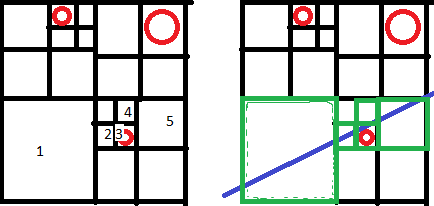
\includegraphics[width=\textwidth]{figures/octreetwod.png}
	\caption{Visualization of the collision tests a ray traveling trough an octree data structure.}
	\label{fig:octreetraversal}
\end{figure}

\subsection{Octree}
Collisions against the octree uses a iterative solution to traverse a ray trough the tree.
When a ray is created, it is compared against all the top boxes.
As the ray is evaluated, the bounding box closest to the ray are found, iterating down.
If no collisions is found, the algorithm iterates up again, finding the smallest neighbouring bounding box that has data in it. This process is visualized in \autoref{fig:octreetraversal}. The ray first collides with bounding box 1, but no child nodes exist in it, so the ray traverse forward to the edge of bounding box 2 as it collides with the sibling to 1. 
It now iterates down to bounding box 2 in the figure and finds that no child's are in this bounding box. 
The ray moves forward to bounding box 3 and finds a primitive in this bounding box, collision tests are done against it but no collision is found.
The ray traverse forward to the edge of bounding box 3 and trough bounding box 4.
The ray exits out of bounding box 5 and no collisions were found and therefore, no collisions between the scene and the ray were found.\\

This allows for using the fast and cheap AABB intersection method instead of expensive collision tests using all primitives.

\section{Anti-aliasing by sub-pixel sampling}
To reduce aliasing effects in the final image we have implemented support for sub-pixel sampling.
This means that instead of sending one view ray from the virtual camera through the center of a pixel on the view plane, we send several view rays distributed on the pixel and average their results.
The view ray distribution on a pixel area can be done in a uniform random fashion or simply placed linearly evenly spaced.
For all rendered images in this report, the uniform random distribution was used.
In  \autoref{fig:antialiasing} we see a comparison between using 1 view ray per pixel on the left, and 10 view rays per pixel on the right.

\begin{figure}
        \centering
        \begin{subfigure}[b]{0.3\textwidth}
                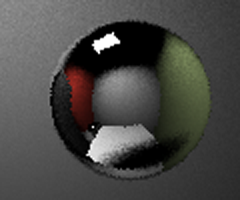
\includegraphics[width=\textwidth]{figures/aliasing_1.png}
                \caption{1 view ray per pixel}
                \label{fig:aliasing1}
        \end{subfigure}%
        ~ %add desired spacing between images, e. g. ~, \quad, \qquad etc.
          %(or a blank line to force the subfigure onto a new line)
        \begin{subfigure}[b]{0.3\textwidth}
                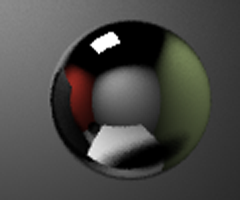
\includegraphics[width=\textwidth]{figures/aliasing_10.png}
                \caption{10 view rays per pixel}
                \label{fig:aliasing10}
        \end{subfigure}
        \caption{Antialising by randomly distributed sub-pixel sampling}\label{fig:antialiasing}
\end{figure}

\section{Russian Roulette}
Russian roulette is a method for ray termination that specifies a probability for continuing or terminating at each bounce. 
How the probability is decided depends on how complex the implementation.
A simple implementation only states a fixed threshold of probability for each ray.
As the ray continues forward, the probability of terminating increases.
More complex implementations could use reflectance of the surface to decide, giving a higher probability of termination for diffuse primitives.
Light intensity could also be taken into consideration when determining the probability, giving a higher chance of termination for low intensity values.

\section{Monte Carlo ray tracing}
As described in the introduction a Monte Carlo ray tracer is similar to a Whitted ray tracer in that it is only interested in the radiance reaching the virtual camera, or the eye.
It is a complete global illumination algorithm, and solves the rendering equation \autoref{eq:rendering_eq}, repeated below for convenience, by random sampling.

\begin{equation}
L(x \rightarrow \theta) = L_e(x \rightarrow \theta) + \int_{\Omega_x} f_r(x, \Phi \rightarrow \theta)L(x \leftarrow \Phi)cos(N_x, \Phi)d\omega_{\Phi}
\tag{\ref{eq:rendering_eq}}
\end{equation}

The left hand side $L(x \rightarrow \theta)$ corresponds to the radiance leaving at a point \emph{x} in the direction $\theta$.
The right hand side consists of an emmitance part and a reflectance part.
$ L_e(x \rightarrow \theta)$ corresponds to outgoing radiance emmited from $x$, and the integral term corresponds to reflected radiance received from all directions over a hemisphere over the point $x$.
In \cite{dutre} it is shown that \autoref{eq:rendering_eq} can be represented by separating the terms for indirect and direct illumination as in \autoref{eq:rendering_eq_split}.


\begin{subequations} \label{eq:rendering_eq_split}
\begin{align} 
&L(x \rightarrow \theta) = L_{direct}+L_{indirect} \\
&L_{direct}(x \rightarrow \theta) = \int_A L_e(y \rightarrow \mathbf{yx})f_r(x, \mathbf{xy}\rightarrow \theta)G(x,y)V(x,y)dA_y \\
&L_{indirect}(x \rightarrow \theta) = \int_{\Omega_x} L_r(x \leftarrow \Phi) f_r(x, \Phi \rightarrow \theta)cos(N_x, \Phi)d\omega_{\Phi}
\end{align}
\end{subequations}

\subsection{Direct illumination}
The term $L_{direct}(x \rightarrow \theta)$ expresses the contribution to a point \emph{x} from light sources directly.
Since the term $L_{direct}(x \rightarrow \theta)$ contains the emittance term $L_e$ it is only non-zero for light sources, we can describe the direct illumination contribution as in \autoref{eq:rendering_eq_split}b, which is an integral over the area of the light sources in the scene instead of an integral over the hemisphere.
Or as a discrete representation as a sum over all \emph{N} light sources in the scene.
In our implementation only a single planar light source is considered.
For generality's sake all equations presented will be defined to handle an arbitrary number of light sources.

\begin{equation}
\label{eq:disc_direct}
L_{direct}(x \rightarrow \theta) = \sum^{N}_{k=1} \int_{A_k}L_e(y \rightarrow \mathbf{yx}) f_r(x, \mathbf{xy}\leftrightarrow \theta)G(x,y)V(x,y)dA_y
\end{equation}

In \autoref{eq:rendering_eq_split}b, $A$ refers to the area of a light source in the scene.
For every intersection point retrieved from the scene, that point's direct illumination is calculated in two separate ways, one for direct diffuse illumination and one for direct specular illumination.
For diffuse direct illumination the light source is sampled.
Each sample point $y_i$ is distributed uniformly on the surface of the light source.
The visibility function $V(x,y)$ makes sure that only sample points visible from \emph{x} will contribute to the direct illumination by checking if $y_i$ is in line of sight of \emph{x}.
Because of this these rays are often called shadow rays, and will result in soft shadows if enough samples $y_i$ are taken.
For a single planar area light source sampled with $N_s$ shadow rays the Monte Carlo estimator becomes

\begin{equation}
\label{eq:monte_carlo_direct}
\langle L_{direct}(x \rightarrow \theta) \rangle = \frac{1}{N_s} \sum^{N_s}_{i=1} \frac{L_e(y_i \rightarrow \mathbf{y_ix}) f_r(x, \theta \leftrightarrow \mathbf{xy_i})G(x,y_i)V(x,y_i)}{p(y_i)}
\end{equation}
as described in \cite{dutre}.

A uniform probability distribution function $p(y_i)$ of $\frac{1}{A}$ is used where \emph{A} is the area of the light source.
From \autoref{eq:monte_carlo_direct} we see that it is required to evaluate visibility, BRDF and radiance emitted for each sample point.

Direct specular illumination is handled more straight forward.
If a ray intersects with a specular object, a new ray is traced from the intersection point in the direction of a perfect reflection of the first incoming ray.
If this new ray intersects a light source the point at the initial intersection receives radiance contribution in the form of emittance from that light source.

\subsection{Indirect illumintaion}
Indirect illumination corresponds to radiance received through one or more reflections against other objects in the scene.
The contribution from indirect illumination for a point \emph{x} is done by evaluating the integral over the hemisphere in \autoref{eq:rendering_eq_split}c. Unfortunately we cannot transform this expression into an integral over a smaller domain as we did for direct illumination since the reflectance term $L_r$, which in turn contains radiance from other points in the scene, appears on both sides of the equation.
The recursive nature of this algorithm is evident and it is clear that an exact solution is cannot be found.
We instead use a Monte Carlo estimator as presented in \cite{dutre}.

\begin{equation}
\label{eq:monte_carlo_indirect}
\langle L_{indirect}(x \rightarrow \theta) \rangle = \frac{1}{N} \sum^{N}_{i=1} \frac{L_r(r(x,\Phi_i) \rightarrow -\Phi_i) f_r(x, \theta \leftrightarrow \Phi_i)cos(\Phi_i, N_x)}{p(\Phi_i)}
\end{equation}

In \autoref{eq:monte_carlo_indirect} \emph{N} is the number of rays used to sample indirect radiance, $L_r$ is the reflected radiance, $\Phi_i$ is the hemisphere direction of the \emph{i}:th sampled ray, $f_r$ is the BRDF of the surface material of \emph{x}, $N_x$ is the surface normal, and finally $p(\Phi_i)$ is the probability distribution function.
Specular indirect illumination och diffuse indirect illumination are handled separately.

\subsubsection{Diffuse indirect illumination}
In this project all diffuse surfaces are of Lambertian type.
Since a Lambertian diffuse surface per definition reflect equal amounts of radiance in every direction, the BRDF and the pdf for such a surface can both be treated as constants.
We define the BRDF and the pdf for all diffuse surfaces as  in \autoref{eq:diffuse_indirect1}.
\begin{subequations} \label{eq:diffuse_indirect1}
\begin{align} 
&BRDF = \frac{color}{\pi} \\
&p(\Phi_i) = \frac{cos(\Phi_i, N_x)}{\pi}
\end{align}
\end{subequations}

Inserting \autoref{eq:diffuse_indirect1} into \autoref{eq:monte_carlo_indirect} and reducing and realising that constants can be placed outside the sum produces \autoref{eq:diffuse_indirect2}.

\begin{subequations} \label{eq:diffuse_indirect2}
\begin{align}
&\nonumber \frac{1}{N} \sum^{N}_{i=1} \frac{L_r(r(x,\Phi_i) \rightarrow -\Phi_i) f_r(x, \theta \leftrightarrow \Phi_i)cos(\Phi_i, N_x)}{p(\Phi_i)} \rightarrow \\
&\nonumber \frac{1}{N} \sum^{N}_{i=1} \frac{L_r(r(x,\Phi_i) \rightarrow -\Phi_i)  \dfrac{color}{\pi} cos(\Phi_i, N_x)}{\frac{cos(\Phi_i, N_x)}{\pi}} \rightarrow \\
&\frac{color}{N} \sum^{N}_{i=1} L_r(r(x,\Phi_i) \rightarrow -\Phi_i)
\end{align}
\end{subequations}

The random hemisphere sample direction $\Phi_i$ is created by randomly picking two angles $\theta$ and $\phi$, which will represent a sampling direction in spherical coordinates.
The angle $\phi$ is assigned a uniform random value in the interval $[0,2\pi]$ and $\theta$ is assigned a value of $cos^{-1}(r^{ \frac{1}{1+n} })$ where \emph{r} is a uniform random number in the interval $[0,1]$ and \emph{n} is a number in the interval $[0,1]$ which dictates the sample direction's alignment within the cosine lobe around $N_x$. 
Lastly, the sample direction is transformed to Carthesian coordinates and is rotated along $N_x$.

\subsubsection{Specular indirect illumination}
Perfect specular surfaces are implemented in this project.

The BRDF for a specular surface is different from 0 in only a single directon, the perfect reflection direction. 
The BRDF and pdf are defined in equation \autoref{eq:specular_indirect1} where $\theta$ is the incident ray's angle to the surface normal and $\Phi_i$ is the reflected ray angle.
Since we are dealing with perfectly specular materials the pdf will be equal to 1 as well, and $\Phi_i = \theta$ thus the dirac function will yield a result of 1.

\begin{subequations} \label{eq:specular_indirect1}
\begin{align}
	&BRDF = \frac{color}{cos(\Phi_i, N_x)}\delta(\Phi_i - \theta) = \frac{color}{cos(\Phi_i, N_x)} \\
	&pdf = 1
\end{align}
\end{subequations}

Inserting \autoref{eq:specular_indirect1} into \autoref{eq:monte_carlo_indirect} yields

\begin{subequations} \label{eq:specular_indirect2}
\begin{align}
	&\nonumber \frac{1}{N} \sum^{N}_{i=1} \frac{L_r(r(x,\Phi_i) \rightarrow -\Phi_i) f_r(x, \theta \leftrightarrow \Phi_i)cos(\Phi_i, N_x)}{p(\Phi_i)} \rightarrow \\
	&\nonumber \frac{1}{N} \sum^{N}_{i=1} \frac{L_r(r(x,\Phi_i) \rightarrow -\Phi_i) \dfrac{color}{cos(\Phi_i,N_x)} cos(\Phi_i, N_x)}{1} \rightarrow \\
	&\frac{color}{N} \sum^{N}_{i=1} L_r(r(x,\Phi_i) \rightarrow -\Phi_i)
\end{align}
\end{subequations}
which, if $\Phi_i$ does not intersect a light source, is a recursive call that lets the reflected ray continue through the scene.

An intersection with a specular surface can have two results. 
For a specular material that is perfectly opaque, for example a mirror-like material, a reflected ray will be created. 
If the reflected ray in turn does not intersect with a light source it will be recursively iterated and continue through the scene.
If the material instead is not perfectly opaque two rays will be created.
One reflected ray created in the same fashion as described above, and one refracted (transmitted) ray that will continue into the object.
To decide how much of the radiance should be contributed from the reflected ray an approximation of Fresnel's equation as presented by Schlick et al. \cite{schlick} in \autoref{eq:schlicks} is used.

\begin{subequations} \label{eq:schlicks}
\begin{align}
R_0 = \left( \frac{n_1-n_2}{n_1+n_2} \right) ^2 \rightarrow \\
R(\theta) = R_0+ (1-R_0)(1-cos(\theta))^5
\end{align}
\end{subequations}

$R_0$ is the reflection coefficient for light incoming parallel to the normal direction of the surface, $n1$ and $n2$ are the refractive indices for the mediums the ray is come from and going into respectively.
The term $cos(\theta)$ is the dot product between the halfway direction vector and the viewing direction vector. \autoref{eq:schlicks} describes what fraction of the reflected ray should be used in computing the radiance for the intersection point. The radiance contribution from the refracted (transmitted) ray them becomes $T=1-R$.

% TA EJ BORT sparar till senare :P
%\begin{figure}
%        \centering
%        \begin{subfigure}[b]{0.5\textwidth}
%           \includegraphics[width=\textwidth]{figures/2013-12-10-15-39-35-200rpp-ca2h_6-7_112.png}
%	\caption{200 view rays per pixel}
%	\label{fig:full}
%        \end{subfigure}%
%        ~ %add desired spacing between images, e. g. ~, \quad, \qquad etc.
%          %(or a blank line to force the subfigure onto a new line)
%        \begin{subfigure}[b]{0.5\textwidth}
%                \includegraphics[width=\textwidth]{figures/2013-12-10-15-39-35-200rpp-ca2h_6-7_112.png}
%                \caption{HerpDerp view rays}
%                \label{fig:miger}
%        \end{subfigure}
%        \caption{Antialising by randomly distributed sub-pixel sampling}\label{fig:antialiasing}
%\end{figure}

$R_0$ is the reflection coefficient for light incoming parallel to the normal direction of the surface, $n1$ and $n2$ are the refractive indices for the mediums the ray is coming from and going into respectively.
The term $cos(\theta)$ is the dot product between the halfway direction vector and the viewing direction vector.
\autoref{eq:schlicks} describes what fraction of the reflected ray radiance should be used in computing the radiance for the intersection point. 
The radiance contribution from the refracted (transmitted) ray them becomes $T=1-R$.

\subsection{Reflection}
When a ray travels trough a medium, colliding with another medium, the ray will be reflected.
The law of reflection says that the angle of incidence $\theta_i$ is equal to the angle of reflection $ \theta_r $ is equal to each other.
The incoming ray can be divided into two different parts, the tangent part to the surface $ \mathbf{i}_\bot $ and the normal part $ \mathbf{i}_\| $.
The tangiental part can be found using orthogonal projection onto the normal using \autoref{eq:projection}. The normal part is found using \autoref{eq:projectionrest}.

\begin{equation} \label{eq:projection}
\mathbf{i}_\bot = \frac{\mathbf{i} \cdot \mathbf{n}} {\vert \mathbf{n}^2} \mathbf{n} = (\mathbf{v} \cdot \mathbf{n})\mathbf{n}
\end{equation}

\begin{equation} \label{eq:projectionrest}
\mathbf{i}_\| = \mathbf{i} - \mathbf{i}_\bot
\end{equation}
By doing a dot product between these two rays, it is possible to prove that the result is zero and thus proving that these two are orthogonal and that $ \mathbf{i}_\bot $ is an orthogonal projection on $ \mathbf{n} $. By combining \autoref{eq:projectionrest} and \autoref{eq:projection} the reflected ray $ \mathbf{r} $ can be calculated using \autoref{eq:reflectioncalc}.

\begin{subequations}\label{eq:reflectioncalc}
\begin{align}
r =& \mathbf{i}_\| - \mathbf{i}_\bot \\
  =& [\mathbf{i} - (\mathbf{i} \cdot \mathbf{n})\mathbf{n}] - (\mathbf{i} \cdot \mathbf{n}) \mathbf{n} \\
  =& \mathbf{i} - 2 ( \mathbf{i} \cdot \mathbf{n} ) \mathbf{n}
\end{align}
\end{subequations}

%\begin{subequations} \label{eq:refl}
%\begin{align}
%\vert \mathbf{r}_\bot \vert =& cos \theta_r = \theta_i = \vert \mathbf{i} \bot \vert \\ 
%\vert \mathbf{r}_\| \vert =& sin \theta_r = sin \theta_i = \vert \mathbf{i}_\| \vert
%\end{align}
%\end{subequations}

\subsection{Refraction}

When calculating refractions, Snell's law are used. It states that the product of the refractive indices and sines of the angles must be equal, as stated in \autoref{eq:snell}.\\

\begin{equation} \label{eq:snell}
\eta_1 sin \theta_i = \eta_2 sin \theta_t
\end{equation}

This equation has a problem, when $ sin \theta_1 > \dfrac{\eta_1}{\eta_2} $
the other term $ sin \theta_2 $ has to be greater then 1. 
This case is what is called total internal reflection.
When calculating the refracted ray $ t $, continued calculation assumes that the condition is not satisfied.\\

The refractored vector is also divided into two parts, just the same as in \autoref{eq:projectionrest} and the norms are calculated first. By taking advantage of the fact that norms and tangents to the plane is equal to the sines in \autoref{eq:snell} it can be rewritten into \autoref{eq:refraction}.

\begin{equation} \label{eq:refraction}
\mathbf{t}_\| = \frac{\eta_1}{\eta_2} \mathbf{i}_\| = \frac{\eta_1}{\eta_2} 
[\mathbf{i} + cos \theta_i \mathbf{n}]
\end{equation}

The tangential calculation uses Pythagoras which gives \autoref{eq:refractiontan}. The combination of these two, described in \autoref{eq:refractiontot} is all that is needed to calculate the refraction vector 

\begin{equation} \label{eq:refractiontan}
\mathbf{t}_\bot = - \sqrt{1 - \vert \mathbf{t}_\| \vert ^2}\mathbf{n}
\end{equation}

\begin{equation} \label{eq:refractiontot}
\mathbf{t} = \frac{\eta_1}{\eta_2} \mathbf{i} + (\frac{\eta_1}{\eta_2} cos \theta_i - \sqrt{1 - \vert \mathbf{t}_\| \vert ^2})\mathbf{n}
\end{equation}

\subsection{Intensity calculations}
After each time the ray hits a change in medium, it will spawn new refraction and reflection rays.
All of the resulting values that are accumulated from each bounce will be added to the total value.
The contributed values from diffuse and specular elements in 

\chapter{Results and benchmarks} \label{ch:results}

\section{Shadow rays}
The quality of the direct diffuse illumination is directly related to the number of shadow rays used to sample the light source from each intersection point. \autoref{fig:shadow_rays} shows images with different number of shadow rays per sample. Notice how the amount of noise on the floor decreases as the number of shadow rays increases. \autoref{tb:shadow_rays} shows the effect the number of shadow rays has on the rendering time.

\begin{figure}
        \centering
        \begin{subfigure}[h]{0.5\textwidth}
           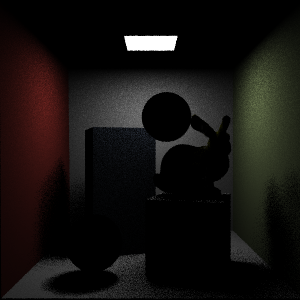
\includegraphics[width=\textwidth]{figures/shadowrays-1-10rpp.png}
	\caption{1 shadow ray}
	\label{fig:1sr}
        \end{subfigure}%
        ~ %add desired spacing between images, e. g. ~, \quad, \qquad etc.
          %(or a blank line to force the subfigure onto a new line)
        \begin{subfigure}[h]{0.5\textwidth}
                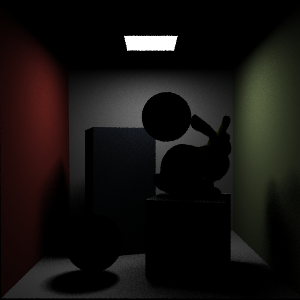
\includegraphics[width=\textwidth]{figures/shadowrays-10-10rpp.png}
                \caption{10 shadow rays}
                \label{fig:10sr}
        \end{subfigure}

	\begin{subfigure}[h]{0.5\textwidth}
                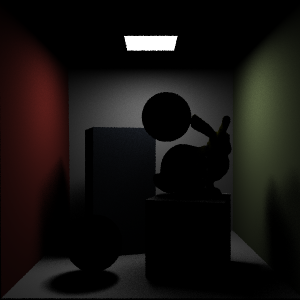
\includegraphics[width=\textwidth]{figures/shadowrays-20-10rpp.png}
                \caption{20 shadow rays}
                \label{fig:20sr}
        \end{subfigure}%
	~
	\begin{subfigure}[h]{0.5\textwidth}
                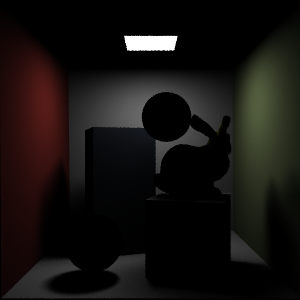
\includegraphics[width=\textwidth]{figures/shadowrays-80-10rpp.png}
                \caption{80 shadow rays}
                \label{fig:80sr}
        \end{subfigure}
        \caption{Number of shadow rays increasing from left to right, top to bottom.}\label{fig:shadow_rays}
\end{figure}

\begin{table}[h]
\begin{center}

	\begin{tabular}{| l | l |}
		\hline
		Shadow rays & Time \\ \hline
		1 & 6s \\ \hline
		10 & 20s \\ \hline
		20 & 34s \\ \hline
		80 & 126s \\ \hline
	\end{tabular}
	\caption{Rendering time for shadow rays.}
	\label{tb:shadow_rays}
\end{center}
\end{table}

\section{Recursion depth}
Recursion depth refers to the number of recursive calls allowed in the algorithm, e.g. how many bounces a ray will make in the scene before terminating and returning. 
The recursion depth affects the noise in the final image, but it also has an impact on the resulting reflections and refractions for specular objects.
As seen in \autoref{fig:recursion_depth} a recursion depth of 0 results in only direct illumination present.
Notice how all specular objects are void of any indirect illumination since only once bounce per ray is allowed. 
A recursion depth of 1 yields slightly better results.
We now see objects that are opaque and specular since rays are allowed to bounce once before termination.
Notice that the glass sphere is still void of indirect illumination since a refraction occurrence involves at least 2 recursive iterations.
A depth of 2 recursions allows for a single refraction instance and the glass sphere is now better represented.
Lastly a render depth of 6 is shown in \autoref{fig:6rd}. This is the recursion depth used for most of the images in this report.
\autoref{tb:recursion} show the effect recursion depth has on rendering time.
\begin{figure}
        \centering
        \begin{subfigure}[h]{0.5\textwidth}
           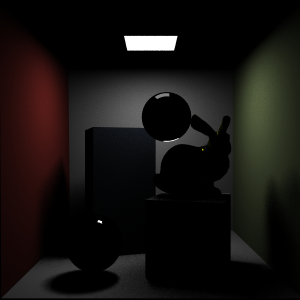
\includegraphics[width=\textwidth]{figures/recursive_depth/recursion-1-100rpp.png}
	\caption{0 recursions}
	\label{fig:1rd}
        \end{subfigure}%
        ~ %add desired spacing between images, e. g. ~, \quad, \qquad etc.
          %(or a blank line to force the subfigure onto a new line)
        \begin{subfigure}[h]{0.5\textwidth}
                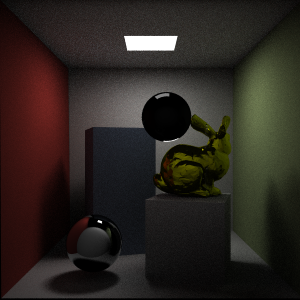
\includegraphics[width=\textwidth]{figures/recursive_depth/recursion-2-100rpp.png}
                \caption{1 recursion}
                \label{fig:2rd}
        \end{subfigure}

	\begin{subfigure}[h]{0.5\textwidth}
                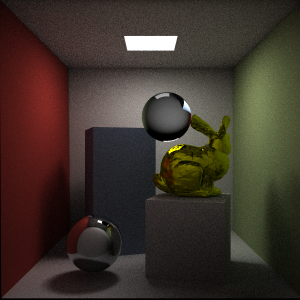
\includegraphics[width=\textwidth]{figures/recursive_depth/recursion-3-100rpp.png}
                \caption{2 recursions}
                \label{fig:3rd}
        \end{subfigure}%
	~
	\begin{subfigure}[h]{0.5\textwidth}
                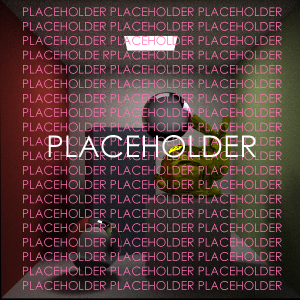
\includegraphics[width=\textwidth]{figures/recursive_depth/recursion-6-1000rppTMP.png}
                \caption{6 recursions}
                \label{fig:6rd}
        \end{subfigure}
        \caption{Increasing recursion depth from left to right, top to bottom.}\label{fig:recursion_depth}
\end{figure}

\begin{table}[h]
\begin{center}
	\begin{tabular}{| l | l |}
		\hline
		Recursion depth & Time \\ \hline
		0 & 11s \\ \hline
		1 & 17s \\ \hline
		2 & 24s \\ \hline
		6 & 55s \\ \hline
	\end{tabular}
	\caption{Rendering time for different recursion depths.}
	\label{tb:recursion}
\end{center}
\end{table}

\begin{figure}
        \centering
        \begin{subfigure}[h]{0.5\textwidth}
           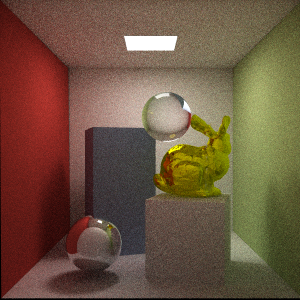
\includegraphics[width=\textwidth]{figures/specular_50rpp-.png}
	\caption{50 view rays per pixel}
	\label{fig:50rpp}
        \end{subfigure}%
        ~ %add desired spacing between images, e. g. ~, \quad, \qquad etc.
          %(or a blank line to force the subfigure onto a new line)
        \begin{subfigure}[h]{0.5\textwidth}
                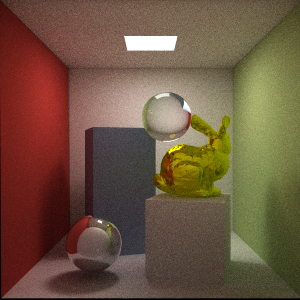
\includegraphics[width=\textwidth]{figures/specular_100rpp-.png}
                \caption{100 view rays per pixel}
                \label{fig:100rpp}
        \end{subfigure}

	\begin{subfigure}[h]{0.5\textwidth}
                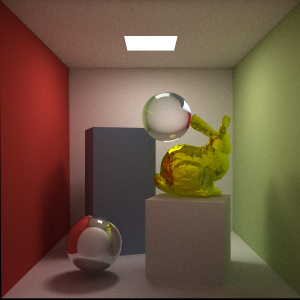
\includegraphics[width=\textwidth]{figures/specular_600rpp-.png}
                \caption{600 view rays per pixel}
                \label{fig:600rpp}
        \end{subfigure}%
	~
	\begin{subfigure}[h]{0.5\textwidth}
                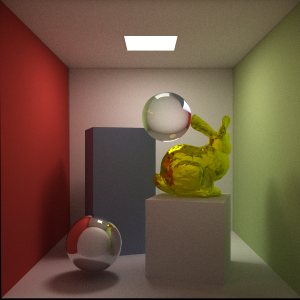
\includegraphics[width=\textwidth]{figures/specular_1000rpp.png}
                \caption{1000 view rays per pixel}
                \label{fig:1000rpp}
        \end{subfigure}
        \caption{Reducing noise by increasing the number of view rays.}\label{fig:vew_rays}
\end{figure}

\section{Noise introduced by specular materials}
Specular materials that produce reflected and to some extent refracted rays is and additional source for noise in the final image and require more samples to reach the same quality level as a scene with only diffuse samples.

\begin{figure}
        \centering
        \begin{subfigure}[b]{0.65\textwidth}
                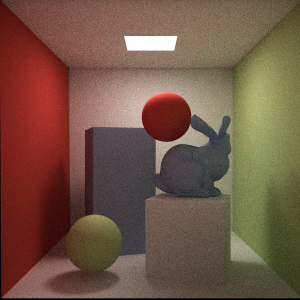
\includegraphics[width=\textwidth]{figures/diffuse-100rpp-.png}
                \caption{Diffuse materials only}
                \label{fig:diff_spec1}
        \end{subfigure}%
         %add desired spacing between images, e. g. ~, \quad, \qquad etc.
          %(or a blank line to force the subfigure onto a new line)

        \begin{subfigure}[b]{0.65\textwidth}
                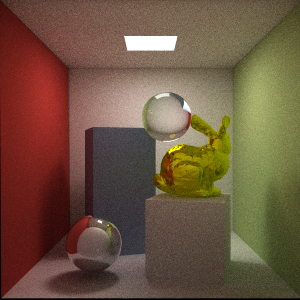
\includegraphics[width=\textwidth]{figures/specular_100rpp-.png}
                \caption{Specular and diffuse materials}
                \label{fig:dif_spec2}
        \end{subfigure}
        \caption{Scene rendered with the same resolution, recursion depth, shadow rays, and a low number of samples per pixel to illustrate the increased noise when specular objects are used in a scene.}\label{fig:diff_spec_diff}
\end{figure}

Notice the increased noise on the surface of the back wall and on the box nearest to the camera in \autoref{fig:diff_spec_diff}.

\section{Samples per pixel}
Another way of reducing the noise in the images is by sending several rays through the same pixel from the camera. 
Instead of sending a single ray through the center of the pixel we send multiple rays placed in the pixel in a uniform random fashion. 
The contributions from each view ray are summed up and normalized to form the final intensity value for the pixel. 
This technique is sometimes referred to as sub-pixel sampling. In \autoref{fig:vew_rays} we see a scene rendered with an increasing amount of view rays per pixel from left to right, top to bottom. 
Notice how the noise seen on the back wall in \autoref{fig:vew_rays}a subsides rather quickly, while the noise in areas not directly visible to the light source persists much longer even though the number of samples increase.


\begin{figure}
         \centering
         \begin{subfigure}[b]{0.5\textwidth}
            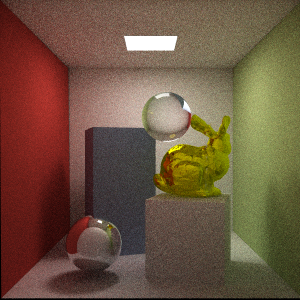
\includegraphics[width=\textwidth]{figures/specular_50rpp-.png}
   \caption{50 view rays per pixel}
   \label{fig:50rpp}
         \end{subfigure}%
         ~ %add desired spacing between images, e. g. ~, \quad, \qquad etc.
           %(or a blank line to force the subfigure onto a new line)
         \begin{subfigure}[b]{0.5\textwidth}
                 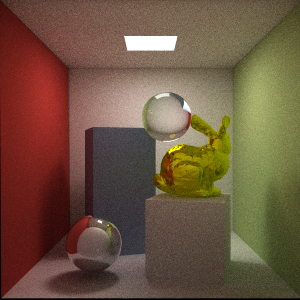
\includegraphics[width=\textwidth]{figures/specular_100rpp-.png}
                 \caption{100 view rays per pixel}
                 \label{fig:100rpp}
         \end{subfigure}
 
   \begin{subfigure}[b]{0.5\textwidth}
                 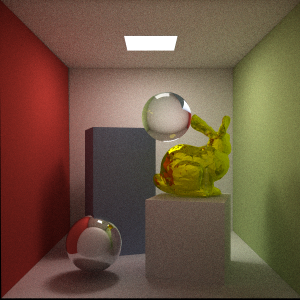
\includegraphics[width=\textwidth]{figures/specular_200rpp-.png}
                 \caption{200 view rays per pixel}
                 \label{fig:200rpp}
         \end{subfigure}%
  ~
  \begin{subfigure}[b]{0.5\textwidth}
                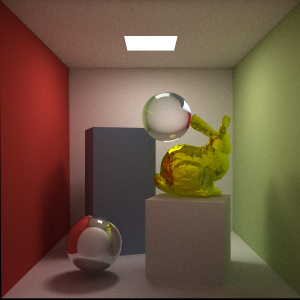
\includegraphics[width=\textwidth]{figures/specular_600rpp-.png}
                \caption{600 view rays per pixel}
                \label{fig:600rpp}
       \end{subfigure}
        \caption{Reducing noise by increasing the number of view rays.}\label{fig:vew_rays}
\end{figure}

\chapter{Discussion} \label{ch:discussion}
Prata t.ex om olika källor för noise. For shadowrays sa skapar var pdf av 1/A en del noise, las om det i boken t.ex.
\emph{Here you should repeat the key findings of your article and discuss how you could improve them. 
Do not go into details, but just give a general description. 
Do not use bullet points. 
You can also give an outlook on how your renderer could be improved etc. 
Length: about 1 page .}

\bibliographystyle{abbrv}
\bibliography{bibl}

\end{document}
